\scanpage{13}
\mspage{10}
Or si $i\leq n$, on aura
\[
\left\{\quad\Lambda\pi_{i0}=0,\qquad\Lambda\pi_{i\alpha}=L^{\unsure{\alpha-1}}w_{i-2\alpha}L^{n-i+\alpha}\pi_{i\alpha}\quad\text{si }\alpha\geq1,\right.
\tag{6.12}
\]
\deleted{et si $j>n$, on aura
\[
\Lambda\pi_{j\alpha}=L
\tag{6.12}
\]}
\[
\Lambda\pi_{2n-i,\alpha}=L^{n-i+\unsure{\alpha}-1}w_{i-2\alpha}\deleted{\unsure{\pi_{2n-i,\alpha}}}L^\alpha\pi_{2n-i,\alpha}\quad(\text{si }i\unsure{\leq|<}n-1)
\tag{6.13}
\]
\margin{Les conditions envisagées impliquent évidemment (iv) : prouver que (iv) implique (ii). Il suffit de prouver en fait que l'on a alors $\pi_i=\pi'_i$. \uline{Démonstration à fournir.}}

\uline{Remarque} Voici un système de conditions déterminant de façon unique les éléments $\Lambda\in\mathcal E^{\unsure{(2)|(-2)}},\ \pi_{i,\alpha}\in\mathcal E^{(0)}$ en termes de $L$, et des $\pi_i\deleted{\unsure{\alpha}}$ (dont nous avons déjà une caractérisation intrinsèque par ailleurs, en termes de l'anneau gradué $\mathcal E$) :
\margin{\deleted{$\unsure{\pi_{2n-i}}$}}
\[
\left\{\begin{aligned}
\textcircled{1}\quad &(\Lambda^{n-i}L^{n-i}-1)\pi_i=0
\qquad\textcircled{2}\quad\deleted{\unsure{\pi_{2n-i}}}(L^{n-i}\Lambda^{n-i}-1)\deleted{\unsure{\pi_{2n-i}}}\pi_{2n-i}=0\\
\textcircled{3}\quad &\pi_{i,\alpha}=L^\alpha\deleted{\unsure{w_{i-2\alpha}}}\inserted{\Lambda^{n-i+2\alpha}}L^{n-i+\alpha}\bigl(1-\sum_{\alpha'>\alpha}\pi_{i,\alpha'}\bigr)\\
\textcircled{4}\quad &\pi_{2n-i,\alpha}=L^{n-i}\pi_{i,\alpha}\Lambda^{n-i}\\
&\deleted{\Lambda=\sum_{j,\alpha}\Lambda\pi_{j\alpha}}\\
\textcircled{5}\quad &\Lambda\pi_{i,0}=0\qquad\deleted{\unsure{\alpha}}\\
\textcircled{6}\quad &\Lambda\pi_{i\alpha}=L^{\alpha-1}\Lambda^{n-i+2\alpha}L^{n-i+\alpha}\pi_{i\alpha}\quad\text{si }\alpha\geq1\\
\textcircled{7}\quad &\Lambda\pi_{2n-i,\alpha}=L^{n-i+\alpha-1}\Lambda^{n-i+2\alpha}L^\alpha\pi_{2n-i,\alpha}\quad\text{si }\unsure{\alpha|i}\leq n-1\\
\textcircled{8}\quad &\Lambda=\sum_{j,\alpha}\Lambda\pi_{j\alpha}
\end{aligned}\right.
\tag{6.14}
\]
(dans ttes ces formules, on suppose $i\leq n$).

Dans ces huit formules, on peut d'ailleurs remplacer les quatre dernières par les suivantes \inserted{\figure{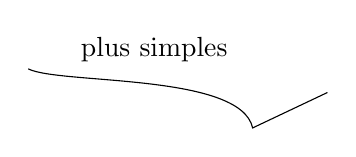
\begin{tikzpicture}[x=1cm,y=1cm]
\node at (0,.35) {plus simples};
\draw (-1.6,.1) .. controls (-1.2,-.1) and (1.1,.05) .. (1.25,-.65) -- (2.2,-.2);
\end{tikzpicture}}} :
\mspage{12}
